\documentclass[11pt, oneside]{article}   	% use "amsart" instead of "article" for AMSLaTeX format


% \usepackage{draftwatermark}
% \SetWatermarkText{Draft}
% \SetWatermarkScale{5}
% \SetWatermarkLightness {0.95} 
% \SetWatermarkColor[rgb]{0.7,0,0}


\usepackage{geometry}                		% See geometry.pdf to learn the layout options. There are lots.
\geometry{letterpaper}                   		% ... or a4paper or a5paper or ... 
%\geometry{landscape}                		% Activate for for rotated page geometry
%\usepackage[parfill]{parskip}    		% Activate to begin paragraphs with an empty line rather than an indent
\usepackage{graphicx}				% Use pdf, png, jpg, or eps� with pdflatex; use eps in DVI mode
								% TeX will automatically convert eps --> pdf in pdflatex		
\usepackage{amssymb}
\usepackage{mathrsfs}
\usepackage{hyperref}
\usepackage{url}
\usepackage{authblk}
\usepackage{amsmath}
\usepackage{graphicx}
\usepackage{fixltx2e}
\usepackage{hyperref}
\usepackage{alltt}
\usepackage{color}
\usepackage{bigints}

\newcommand{\argmax}{\operatornamewithlimits{argmax}}
\newcommand{\argmin}{\operatornamewithlimits{argmin}}

\title{Notes on MSE Gradients for Neural Networks}
\author{David Meyer \\ dmm@\{1-4-5.net,uoregon.edu,...\}}
% \date{17 Jan 2016}


\begin{document}
\maketitle

\section{Introduction}

\section{Mean Squared Error (MSE)}
\noindent
First, notation: scalars are represented in regular math font, e.g., $y_i$, where vectors are in bold, e.g., $\mathbf{x}_i$. Given these definitions we can define our \emph{labelled data} or \emph{training examples} as a set of $n$ tuples where the $i^\text{th}$ tuple has the form $(\mathbf{x}_i,y_i)$, where $\mathbf{x}_i \in \mathbb{R}^n$ is a vector of inputs and $y_i \in \mathbb{R}$ is the observed output.

\bigskip
\noindent
Ideally our neural network should output $y_i$ when given $\mathbf{x}_i$ as an input. Of course, during training this doesn't always happen so we need to define an \emph{error or cost} function that quantifies the difference between the actual observed output and the prediction of the neural network. A simple measure of the error is the Mean Squared Error, or MSE.  We define the MSE as follows:

\begin{flalign}
E := \frac{1}{m} \sum\limits_{i = 1}^{m} (h(\mathbf{x}_i) - y_i)^2
\end{flalign}

\bigskip
\noindent
where $h(\mathbf{x}_i)$ is the output of the neural network.

\section{Basic Building Blocks: Perceptrons}
\noindent
The simplest classifiers out of which we will build our neural network are perceptrons \cite{Rosenblatt1958}. In reality, a perceptron is a linear classifier.   A perceptron takes an input vector $\mathbf{x}$ which is multiplied pairwise by  a weight vector $\mathbf{w}$, then sums the products up together with a bias term $b$. This sum (the \emph{dot product}, Equation \ref{eqn:dot_product}) is then fed through  an activation function $\sigma:\mathbb{R} \rightarrow \mathbb{R}$. This is depicted in Figure \ref{fig:perceptron}.  Note here that $w_0 = b$ and $a_0 = 1$;  I like Figure \ref{fig:perceptron} but I will use the more conventional $\mathbf{x}$ for the input vector  rather than $\mathbf{a}$ as is used in the figure.  The behavior of the perceptron can then be described as $\sigma(\mathbf{w} \cdot \mathbf{x})$, where $\mathbf{w}$ and $\mathbf{x}$ have the following form\footnote{Again noting that $\mathbf{a}$ in Figure \ref{fig:perceptron} is frequently
called $\mathbf{x}$, the input vector; I'll use $\mathbf{x}$ here.}:

\begin{flalign*}
\boldsymbol{w}  & = \begin{bmatrix}  w_{1}  \\ w_{2} \\  \vdots \\ w_{n}   \end{bmatrix}  \\ \\
\boldsymbol{x}   & = \begin{bmatrix}  x_{1}  \\  x_{2}   \\ \vdots \\  x_{n}   \end{bmatrix}
\end{flalign*}

\bigskip
\noindent
$\mathbf{w}^\text{T}$ ($\mathbf{w}$ transpose) is defined to be

\begin{flalign*}
\boldsymbol{w}^T  & = \begin{bmatrix}  w_{1}, & w_{2}, & \hdots, &  w_{n}  \end{bmatrix}
\end{flalign*}


\bigskip
\noindent
The  \emph{dot product} between $\mathbf{w}$ and $\mathbf{x}$, $\mathbf{w} \cdot \mathbf{x}$, is defined as

\begin{equation*}
\label{eqn:dot_product}
\mathbf{w} \cdot \mathbf{x} = \boldsymbol{w}^T\boldsymbol{x} = 
\left[\begin{array}{cccc} w_{1}, & w_{2}, & \cdots, & w_{n} \end{array} \right]  
\left[ \begin{array}{cccc} x_1 \\ x_2 \\ \vdots \\ x_n \end{array} \right] =
\sum\limits_{i = 1}^{n}w_{i}x_{i} = w_{1}x_1 + w_{2}x_2 +  \ldots + w_{n}x_n
\end{equation*}

\bigskip
\noindent
Note that the weight vector, $\mathbf{w}$ will be a $M \times N$ matrix if there is more than one layer of artificial neurons.

\bigskip
\noindent
The last piece of the puzzle are the kinds of activation functions\footnote{Activation functions are sometimes called \emph{link} functions in a Generalized Linear Model setting.} that $\sigma$ might be:
\begin{itemize}
\item Sigmoid: $\sigma(x) = \frac{1}{1+e^{-x}}$
\item Hyperbolic tangent: $\sigma(x) = \tanh(x)$
\item Linear: $\sigma(x) = x$
\item  Rectified Linear Unit: $\sigma(x) = \max(0,x)$
\item  Exponential Linear Unit: 
$\sigma(x) =\left \{ 
        \begin{array}{ll}
		x   & \text{if } x \ge 0 \\
		a(e^x - 1)     & \text{otherwise }
	\end{array}
\right. $
\item ...
\end{itemize}

\begin{figure}
\center{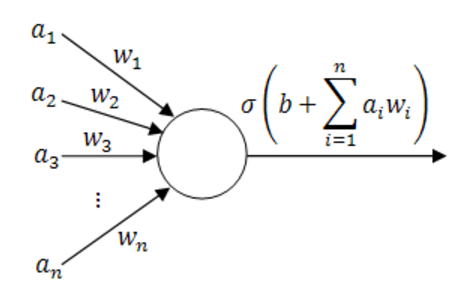
\includegraphics[scale=0.8] {images/perceptron.png}}
\caption{Basic Perceptron/Linear Classifier}
\label{fig:perceptron}
\end{figure}

\section{Building a Single Layer Neural Network}
\noindent
So far we've defined the error $E$ as the MSE, namely, $E := \frac{1}{m} \sum\limits_{i = 1}^{m} (h(\mathbf{x}_i) - y_i)^2$. Here both the error and the output of the network 
($h_{\mathbf{w}}(\mathbf{x}_i) = \sigma(\mathbf{w} \cdot \mathbf{x}_i)$) depend on the weight vector $\mathbf{w}$. We write the error function, parameterized by $\mathbf{w}$, as

\begin{flalign}
E(\mathbf{w}) := \frac{1}{m} \sum\limits_{i = 1}^{m} (h_{\mathbf{w}}(\mathbf{x}_i)  - y_i)^2
\end{flalign}

\bigskip
\noindent
Now, our goal is to find a weight vector $\mathbf{w}$ such that $E(\mathbf{w})$ is minimized. In effect this means that the perceptron will correctly predict the output for the inputs in the training set. Of course, we want the perceptron to  \emph{generalize}, so that it makes correct predictions on the test set and on new examples. But how to do this
minimization?


\begin{figure}
\center{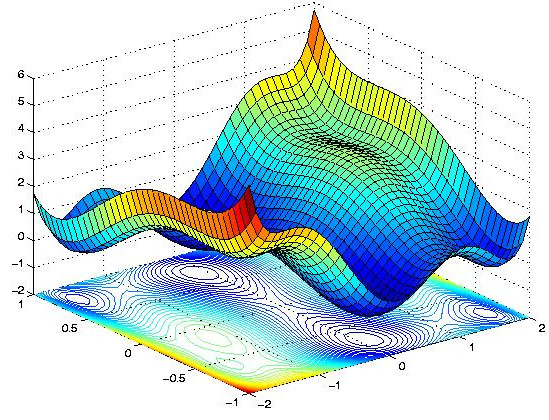
\includegraphics[scale=0.65] {images/optimization.jpg}}
\caption{Non-Convex Error Surface}
\label{fig:non-convex}
\end{figure}

\bigskip
\noindent
We do the minimization by applying the \emph{gradient descent} algorithm.  In effect we will treat the error as a surface in $n$-dimensional space and search for the greatest downwards slope at the current point $\mathbf{w}_t$ and will go in that direction to obtain $\mathbf{w}_{t+1}$. Following this process we will hopefully find a minimum point on the error surface and we will use the coordinates of that point as the final weight vector\footnote{Consider, however, the situation in which the error surface is non-convex, such as is in Figure \ref{fig:non-convex}.}. In any event, the update rule can be stated as follows (in both \emph{partial derivative} and \emph{gradient} notations):

\begin{flalign}
\mathbf{w}_{t+1} & := \mathbf{w}_t - \eta \frac{\partial E(\mathbf{w})}{\partial{\mathbf{w}}} 
\quad \qquad \qquad  \mathbin{\#} \text{partial derivative notation} \\
\mathbf{w}_{t+1} & := \mathbf{w}_t - \eta \nabla_{\mathbf{w}} E(\mathbf{w}) 
\:  \qquad \qquad  \mathbin{\#} \text{gradient (nabla) notation} 
\end{flalign}

\bigskip
\noindent
where $\eta$ is the \emph{learning rate}. Now, notice that the \emph{gradient} of $E$ on $w$ is

\begin{flalign}
\nabla_{w} E(\mathbf{w}) = \frac{\partial E(\mathbf{w})}{\partial{\mathbf{w}}} = \Bigg[\frac{\partial E(\mathbf{w})}{\partial{\mathbf{w_0}}}, 
\frac{\partial E(\mathbf{w})}{\partial{\mathbf{w_1}}}, \cdots,  \frac{\partial E(\mathbf{w})}{\partial{\mathbf{w_n}}} \Bigg ]
\end{flalign}

\bigskip
\noindent
Now we can calculate the gradient, $\nabla_{\mathbf{w}} E(\mathbf{w})$.  We start by calculating $\frac{\partial E(\mathbf{w})}{\partial{\mathbf{w_j}}}$ for each $j$.  So first....
Note that the \emph{chain rule} states that if $h(x) = f(g(x))$ then the derivative $\frac{d h(x)}{dx} = h^\prime(x) = f^\prime(g(x)) g^\prime(x)$.  We will also use the \emph{power rule}: If $y = u^n$, then $\frac{dy}{dx} = n u^{n-1} \frac{du}{dx}$. So the partial derivative $\frac{\partial E(\mathbf{w})}{\partial{\mathbf{w_j}}}$ can be computed as follows: So for example element of the gradient $0 \le j \le n$

\begin{flalign}
\frac{\partial E(\mathbf{w})}{\partial{\mathbf{w_j}}} & = \frac{\partial}{\partial w_j}
\frac{1}{m}\sum\limits_{i = 1}^m (h_{\mathbf{w}}(\mathbf{x}_i) - y_i)^2 
 \qquad \qquad \qquad \qquad  \qquad \mathbin{\#} \text{definition of } E\\
&=\frac{1}{m}\ \sum\limits_{i = 1}^m 2 (h_{\mathbf{w}}(\mathbf{x}_i) - y_i) \frac{\partial}{\partial w_j} (h_{\mathbf{w}}(\mathbf{x}_i) - y_i)  \qquad \quad \:  \: \mathbin{\#} \text{power rule} \\
&= \frac{1}{m}\ \sum\limits_{i = 1}^m 2 (h_{\mathbf{w}}(\mathbf{x}_i) - y_i) \frac{\partial}{\partial w_j} \sigma(\mathbf{w} \cdot \mathbf{x}_i)  \; \quad \qquad \qquad  \mathbin{\#} h_{\mathbf{w}}(\mathbf{x}_i) = \sigma(\mathbf{w} \cdot \mathbf{x}_i) \\
&= \frac{1}{m}\ \sum\limits_{i = 1}^m 2 (h_{\mathbf{w}}(\mathbf{x}_i) - y_i) \sigma^\prime (\mathbf{w} \cdot \mathbf{x}_i)  \frac{\partial}{\partial w_j} \mathbf{w} \cdot \mathbf{x}_i  \: \:  \qquad  \mathbin{\#} \text{chain rule} \\
&= \frac{1}{m}\ \sum\limits_{i = 1}^m 2 (h_{\mathbf{w}}(\mathbf{x}_i) - y_i) \sigma^\prime (\mathbf{w}  \cdot \mathbf{x}_i)\frac{\partial}{\partial w_j} \sum\limits_{k =1}^{n} w_k x_{i,k}  \:  \mathbin{\#} \text{defn dot product} \\
&= \frac{1}{m}\ \sum\limits_{i = 1}^m 2 (h_{\mathbf{w}}(\mathbf{x}_i) - y_i) \sigma^\prime (\mathbf{w} \cdot \mathbf{x}_i) x_{i,j}   \qquad \quad \quad \quad   \mathbin{\#} \frac{\partial w_k x_{i,k}}{\partial w_j} \ne 0 \text { when } k = j
\end{flalign}

\bigskip
\noindent
Note that going from Equation 7 to Equation 8 uses the \emph{sum rule}

\bigskip
\begin{flalign}
\frac{d}{dx} (f(x) + g(x)) &= \frac{d}{dx} f(x) + \frac{d}{dx} g(x)
\end{flalign}

\bigskip
\noindent
Here $f(x) = h_{\mathbf{w}}(\mathbf{x}_i)$ and $g(x) = -y_i$. $\frac{\partial}{\partial w_j} h_{\mathbf{w}}(\mathbf{x}_i) = \frac{\partial}{\partial w_j}  \sigma(\mathbf{w} \cdot \mathbf{x}_i)$ and $\frac{\partial y_i}{\partial w_j} = 0$, so we're left with term  $\frac{\partial}{\partial w_j} \sigma(\mathbf{w} \cdot \mathbf{x}_i)$ as we see in Equation 8.

\bigskip
\noindent
Now, using the sigmoid activation function $\sigma(x) = \frac{1}{1+e^{-x}}$, who's derivative 
$\sigma^\prime(x) = \sigma(x) (1 - \sigma(x))$, gives us
\begin{flalign}
\frac{\partial E(\mathbf{w})}{\partial{\mathbf{w_j}}} 
& = \frac{2}{m} \sum\limits_{i = 1}^m (h_{\mathbf{w}}(\mathbf{x}_i) - y_i)  \sigma^\prime (\mathbf{w} \cdot \mathbf{x}_i) x_{i,j}  \\
&=  \frac{2}{m} \sum\limits_{i = 1}^m (\sigma(\mathbf{w} \cdot \mathbf{x}_i) -y_i) \sigma(\mathbf{w} \cdot \mathbf{x})  (1 - \sigma(\mathbf{w} \cdot \mathbf{x})) x_{i,j} \\
\end{flalign}

\noindent
Now, we can compute the gradient $\frac{\partial E(\mathbf{w})}{\partial{\mathbf{w}}}$ as follows:

\begin{flalign}
\frac{\partial E(\mathbf{w})}{\partial{\mathbf{w}}} &=\frac{2}{m} \sum\limits_{i = 1}^m (\sigma(\mathbf{w} \cdot \mathbf{x}_i) -y_i) \sigma(\mathbf{w} \cdot \mathbf{x}_i)  (1 - \sigma(\mathbf{w} \cdot \mathbf{x}_i)) \mathbf{x}_i \\
\end{flalign}

\noindent
Finally, let the update rate $\eta = 0.1$. Then the update to $\mathbf{w}$ is computed as
\begin{flalign}
\mathbf{w}_{t+1} := \mathbf{w}_t - \frac{0.2}{m} \sum\limits_{i = 1}^m (h_\mathbf{w}(\mathbf{x}_i) - y_i) 
h_\mathbf{w}(\mathbf{x}_i ) (1 - h_\mathbf{w}(\mathbf{x}_i ) ) \mathbf{x}_i
\end{flalign}
where $h_\mathbf{w}(\mathbf{x}_i) = \sigma(\mathbf{w}_t \cdot \mathbf{x}_i)$.


\section{What About Multilayer Networks?}

Consider a more general multilayer neural network, such as shown in Figure \ref{fig:multi-layer-perceptron}. Here we are using the notation $w_{i \rightarrow j}$ to denote the weights on the connection between perceptrons $i$ and $j$. I like the $i \rightarrow j$ subscript because it is explicit about direction but will note here that frequently you will see this written as $w_{i, j}$.  That is,  $w_{i \rightarrow j} \equiv w_{i, j}$. Now,  given this notation we can write the sum of the inputs to perceptron (node) $j$ as 

\begin{flalign}
s_j := \sum\limits_{k} z_k w_{k \rightarrow j}
\end{flalign}

\noindent
Here $k$ iterates over all the perceptrons connected to $j$. The output of $j$ is written as $z_j = \sigma (s_j)$, where $\sigma$ is $j$'s activation (link) function.

\bigskip
\noindent
Now, we can use the same error (cost) function for the multlayer network, $E(\mathbf{w})$

\begin{flalign}
E(\mathbf{w}) := \frac{1}{m} \sum\limits_{i = 1}^{m} (h_{\mathbf{w}}(\mathbf{x}_i)  - y_i)^2
\end{flalign}
\noindent
except that now $\mathbf{w}$ is a matrix that contains all the weights for the network: \\
$\mathbf{w} = [w_{i \rightarrow j}] \; \forall i,j$.
 
 \bigskip
 \noindent
The goal is again to find the $\mathbf{w}$ that minimizes $E(\mathbf{w})$ using gradient descent. So we need to calculate $\frac{\partial E(\mathbf{w})}{\partial \mathbf{w}}$. The first step is to separate the contributions of each of the $m$ training examples using the following observation:

\begin{flalign}
\frac{\partial E(\mathbf{w})}{\partial \mathbf{w}} = \frac{1}{m}\sum\limits_{i = 1}^m \frac{\partial E_i(\mathbf{w})}{\partial \mathbf{w}}
\end{flalign}

\noindent
where $E_i(\mathbf{w}) = (h_{\mathbf{w}}(\mathbf{x}_i) - y_i)^2$. Then

\begin{flalign}
\frac{\partial E_i(\mathbf{w})}{\partial w_{j \rightarrow k}} 
&= \frac{\partial}{\partial w_{j \rightarrow k}} (h_{\mathbf{w}}(\mathbf{x}_i) - y_i)^2  \qquad \qquad \qquad \qquad  \: \: \mathbin{\#} \text{definition of } E\\
& = 2 (h_{\mathbf{w}}(\mathbf{x}_i) - y_i) \frac{\partial h_{\mathbf{w}}(\mathbf{x}_i)}{\partial w_{j \rightarrow k}} \\
& = 2 (h_{\mathbf{w}}(\mathbf{x}_i) - y_i) \frac{\partial h_{\mathbf{w}}(\mathbf{x}_i)}{\partial s_k} \frac{\partial s_k}{\partial w_{j \rightarrow k}}  \qquad \quad \quad \quad   \mathbin{\#} \text{chain rule} 
\label{eqn:cr} \\
&= 2 (h_{\mathbf{w}}(\mathbf{x}_i) - y_i) \frac{\partial h_{\mathbf{w}}(\mathbf{x}_i)}{\partial s_k} z_j
\label{eqn:z}
\end{flalign}

\begin{figure}
\center{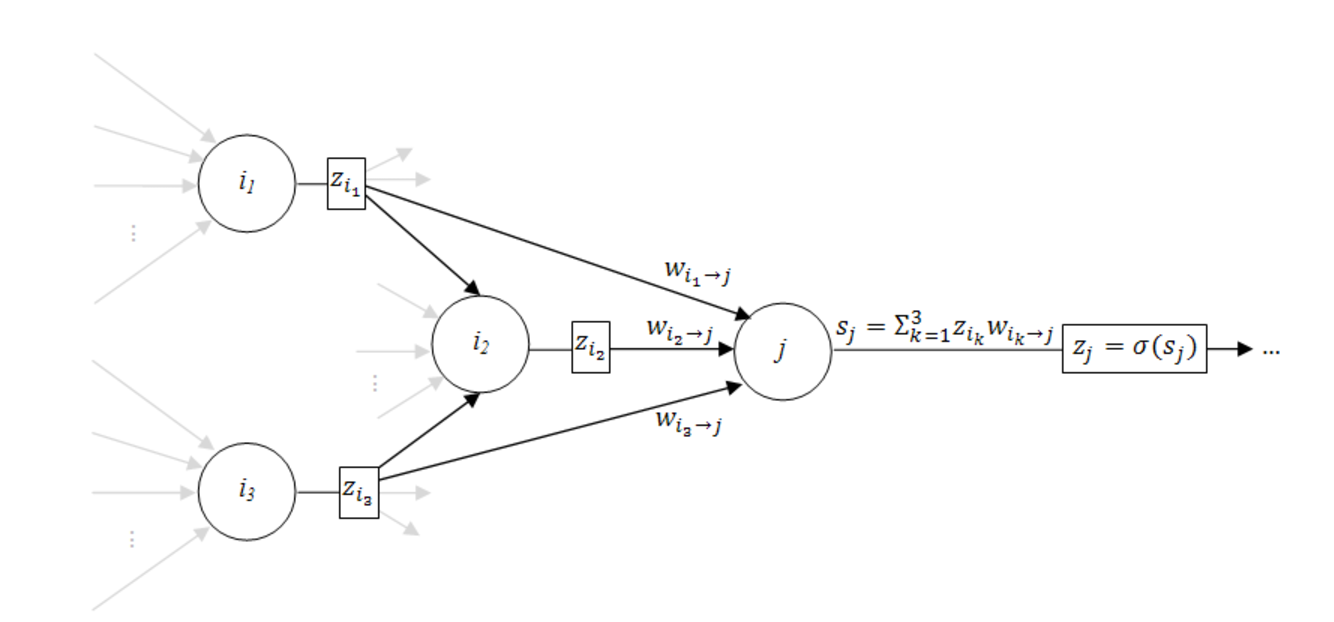
\includegraphics[scale=0.6] {images/multi-layer-perceptron.png}}
\caption{Multi-Layer Perceptron}
\label{fig:multi-layer-perceptron}
\end{figure}



\bigskip
\noindent
Note that in going from Equation \ref{eqn:cr} to  Equation \ref{eqn:z},  $s_k = \sum\limits_{i} z_i w_{i \rightarrow k}$, so $\frac{\partial s_k}{\partial w_{j \rightarrow k}} \ne 0$ where $i = j$ and 0 otherwise.

\bigskip
\noindent
Now, if the $k^\text{th}$ node is an output node,  then
\begin{flalign}
\frac{\partial h_{\mathbf{w}}(\mathbf{x}_i)}{\partial s_k}   
&= \frac{\partial \sigma(s_k)}{\partial s_k}  = \sigma^\prime(s_k)
\end{flalign}

\bigskip
\noindent
so that 
\begin{flalign}
\frac{\partial E_i(\mathbf{w})} {\partial w_{j \rightarrow k}} = 2 (h{\mathbf{w}}(\mathbf{x}_i) -y_i) \sigma^\prime(s_k) z_j
\end{flalign}

\bigskip
\noindent
On the other hand, if $k$ is not an output node, then changes to $s_k$ can affect all the nodes which are connected to $k$'s output, as follows

\begin{flalign}
\frac{\partial h_{\mathbf{w}}(\mathbf{x}_i)}{\partial s_k} &= \frac{\partial h_{\mathbf{w}}(\mathbf{x}_i)}{\partial z_k} \frac{\partial z_k}{\partial s_k}  \qquad \qquad \quad \qquad \qquad \qquad   \mathbin{\#} \text{chain rule again} \\
&= \frac{\partial h_{\mathbf{w}}(\mathbf{x}_i)}{\partial z_k}  \sigma^\prime(s_k)
 \qquad  \qquad \qquad  \qquad \qquad  \mathbin{\#}  z_k = \sigma(s_k) \\
 &= \sum\limits_{o \in \{v \mid v \rightarrow k\}} \frac{\partial h_{\mathbf{w}}(\mathbf{x}_i)}{\partial s_o} \frac{\partial s_o}{\partial z_k} \sigma^\prime(s_k)  \qquad \quad \quad  \:  \mathbin{\#} v \text{ is connected to } k
\label{eqn:zo0} \\
 &= \sum\limits_{o \in \{v \mid v \rightarrow k\}} \frac{\partial h_{\mathbf{w}}(\mathbf{x}_i)}{\partial s_o} w_{k \rightarrow o}  \sigma^\prime(s_k)  \qquad \quad \quad  \:  \mathbin{\#} s_o = \sum\limits_{i} z_i w_{i \rightarrow o}
\label{eqn:zo1}
\end{flalign}

\bigskip
\noindent
Note that in going from Equation \ref{eqn:zo0} to Equation \ref{eqn:zo1} we see that  
\bigskip
\begin{flalign}
\frac{\partial s_o}{\partial z_k} &= \frac{\partial}{\partial z_k} \sum\limits_i z_i w_{i \rightarrow o}
\end{flalign}
\bigskip
\noindent
which is only non-zero when $i = k$, so that $\frac{\partial s_o}{\partial z_k} = w_{k \rightarrow o}$ (Equation \ref{eqn:zo1}).

\noindent
So what is left is to calculate $s_k$ and $z_k$ (feeding forward) and then work backwards from the output calculating 
$\frac{\partial h_{\mathbf{w}}(\mathbf{x}_i)}{\partial s_k}$ and back propagate the error down the network ("backprop"). The summary looks like:

\bigskip
\begin{itemize}
\item $k$ is an output node: $\frac{\partial E_i(\mathbf{w})} {\partial w_{j \rightarrow k}} = 2 (h{\mathbf{w}}(\mathbf{x}_i) -y_i) \sigma^\prime(s_k) z_j$
\item otherwise: $\frac{\partial E_i(\mathbf{w})} {\partial w_{j \rightarrow k}} = 2 (h{\mathbf{w}}(\mathbf{x}_i) -y_i) \sigma^\prime(s_k) z_j \sum\limits_{o \in \{v \mid v \rightarrow k\}} \frac{\partial h_{\mathbf{w}}(\mathbf{x}_i)}{\partial s_o} w_{k \rightarrow o}$
\end{itemize}

\bigskip
\noindent
Using these results we see that

\bigskip
\begin{flalign}
\frac{\partial E_i(\mathbf{w})}{\partial \mathbf{w}} = \Bigg [\frac{\partial E_i(\mathbf{w})} {\partial w_{j \rightarrow k}} \Bigg ] \: \: \forall j,k
\end{flalign}

\bigskip
\noindent
Finally, the weights can be updated in batch mode, in which case the update rule  for batch size of $m$ is
\begin{flalign}
\mathbf{w}_{t+1} & := \mathbf{w}_t - \eta \frac{\partial E(\mathbf{w})}{\partial \mathbf{w}} \\
& := \mathbf{w}_t - \eta \sum\limits_{i = 1}^m \frac{\partial E_i(\mathbf{w})}{\partial \mathbf{w}}
\end{flalign}

\bigskip
\noindent
Or if we take a Stochastic Gradient Descent (SGD) approach (one training example at a time):
\begin{flalign}
\mathbf{w}_{t+1} & := \mathbf{w}_t - \eta \frac{\partial E(\mathbf{w})}{\partial \mathbf{w}} 
\end{flalign}

\bigskip
\section{Acknowledgements}
\noindent 
Thanks to Armin Wasicek for his careful reading of earlier versions of this document.

% \newpage
\bibliographystyle{plain}
\bibliography{/Users/dmm/papers/bib/ml}


\end{document} 

